\documentclass[t]{beamer}

\usetheme{CambridgeUS}
\usecolortheme{beaver}
\setbeamertemplate{navigation symbols}{}

\usepackage[utf8]{inputenc}
\usepackage[croatian]{babel}

\usepackage{datetime}
\renewcommand{\dateseparator}{.}
\newcommand{\todayiso}{\twodigit\day \dateseparator \twodigit\month \dateseparator \the \year}
\date{\todayiso}

\usepackage{listings}
\usepackage{graphicx}
\usepackage{subcaption}
\captionsetup{compatibility=false}
\usepackage{multicol}

\title[NKOSL]{Napredno korištenje operacijskog sustava Linux}
\author[Leonard Volarić Horvat]{Leonard Volarić Horvat\\ {\small Nositelj: doc.dr.sc. Stjepan Groš}}
\subtitle{2. Datotečni sustav, RAID, LVM, kvote}
\institute[FER]{Sveučilište u Zagrebu\\Fakultet elektrotehnike i računarstva}


\begin{document}

{
	\setbeamertemplate{footline}{}
	\begin{frame}
		\maketitle
	\end{frame}
}

\begin{frame}
	\frametitle{Sadržaj}
	\tableofcontents
\end{frame}

\section{Datotečni sustav}

\begin{frame}
	\topskip0pt
	\vspace*{\fill}
		\begin{center}
			\Huge{Datotečni sustav}
		\end{center}
	\vspace*{\fill}
\end{frame}

\begin{frame}
	\frametitle{File system}
	\begin{itemize}
	    \item Datotečni sustav (\textit{file system}) određuje način spremanja i dohvaćanja podataka s medija
		\begin{itemize}
			\item na tvrdom disku određen za svaku particiju
			\item inicijalizacija \textit{formatiranjem}
		\end{itemize}
		\vfill
		\item Funkcionalnosti \textit{file systema}:
		\begin{itemize}
			\item normiranje imena datoteka i upravljanje direktorijima
			\item metadata na datotekama
			\item upravljanje prostorom na mediju:
			\begin{itemize}
				\item smještanje podataka u sektore
				\item grupiranje sektora u blokove
				\item briga o fragmentiranim fajlovima
			\end{itemize}
	    \end{itemize}
	\end{itemize}
\end{frame}

\begin{frame}
	\frametitle{File system}
	\begin{itemize}
		\item \textit{File system} sadrži:
		\begin{itemize}
			\item opisnike fajlova (veličina, lokacija, fragmentacija...)
			\item imena fajlova
			\item hijerarhiju direktorija (npr. FHS)
			\item svoje parametre (npr. veličina bloka)
		\end{itemize}
		\vfill
	    \item Dakle, \textit{file system} je:
	    \begin{itemize}
	    	\item sučelje između bajtova na disku i njihovog grupiranja u smislene cjeline
	    	\item skup metapodataka koji opisuju pohranjene podatke
	    \end{itemize}
    \end{itemize}
\end{frame}




\begin{frame}
	\frametitle{Neki datotečni sustavi}
	\begin{itemize}
		\item FAT - \emph{File Allocation Table}\
		\begin{itemize}
			\item Masovna podrška
			\item FAT12 -\textgreater VFAT -\textgreater FAT16 -\textgreater FAT32 -\textgreater exFAT
			\item Najveća veličina datoteke 4 GiB (FAT32)
		\end{itemize}
		\item ext - \emph{extended filesystem}
		\begin{itemize}
			\item Razvijen za Linux sustave
			\item ext2, ext3, ext4
			\item ext4 danas najčešće korišten
			\item Struktura metapodataka prilagođena Unix file systemu	
			\item Datoteke predstavljene strukturom \emph{inode}
			\item ext3 uvodi \emph{journaling}
		\end{itemize}
	\end{itemize}
\end{frame}


\begin{frame}
	\frametitle{Ostali tipovi}
    \begin{itemize}
        \item ISO 9660
        \item Linear Tape FS
        \item GlusterFS, BGFS
		\item NTFS - danas najčešći FS na modernim Windows verzijama
        \item posebni: swap, tmpfs
    \end{itemize}

    swap
	\begin{itemize}
		\item \emph{Paging} particija
		\item Dio virtualne memorije
	\end{itemize}
	tmpfs
	\begin{itemize}
		\item Spremanje podataka na RAM
		\item Obično montiran na \texttt{/tmp}
	\end{itemize}
\end{frame}


\begin{frame}
	\frametitle{Journaling}
	\begin{itemize}
		\item Bilježenje promjena u FS-u
		\item Drastično se pospješuje robusnost sustava u slučaju kvara:
		\begin{itemize}
			\item veća vjerojatnost uspješnog vraćanja izgubljenih podataka
			\item lakša i puno brža dijagnoza i popravljanje kvara
		\end{itemize}
		\item Konfigurabilna granulacija logova
	\end{itemize}
\end{frame}

\begin{frame}
	\frametitle{inode}
	\begin{itemize}
		\item Struktura koja pohranjuje metapodatke o fajlu
		\item Dozvole, ID vlasnika, GID, veličina, broj hard linkova, MAC vremena
		\item Opaska: ime fajla \textbf{nije} zapisana u inodeu nego u direktoriju
		\begin{itemize}
			\item \emph{Everything is a file!}
			\item direktorij je poseban fajl koji sadrži imena svih fajlova koje (konceptualno) sadrži
		\end{itemize}
		\item Ovakav zapis omogućuje efikasno kopiranje i premještanje fajlova
		\begin{itemize}
			 \item kopiranje: dodavanje novog para (ime,inode) u ciljani direktorij
			 \item premještanje: dodavanje novog para u ciljani i brisanje starog para iz izvornog direktorija
			 \item \textbf{nema potrebe za stvarnim potencijalno dugotrajnim premještanjem sadržaja fajla}
		\end{itemize}
		\item Ispis inodeova: \textit{ls -i}
	\end{itemize}
\end{frame}

\begin{frame}
	\frametitle{ext2}
    Ispod površine ext2fs:

    \begin{itemize}
        \item FS je podijeljen u blokove, 1-4KiB
        \item Blokovi su povezani u blok-grupe, veličine 8-512MiB. 
        \item Svaka grupa sadrži:
        \begin{itemize}
        	\item jedan superblok - podaci o FS
        	\item FS opisnik (sigurnosna redundancija)
        	\item podatke
        \end{itemize}
        \item File je predstavljen strukturom inode (\textit{index node})
        \item indode ima 15 pointera na podatke
        \item Ovisno o veličini blokova restrikcije su
        \item[] \begin{tabular}{l l}
        	Max file size & 16 GiB - 2 TiB \\
        	Max FS size & 4 TiB - 32 TiB
        	\end{tabular}
    \end{itemize}
\end{frame}




\begin{frame}[fragile]
	\frametitle{Upravljanje particijama}
    Stvaranje ext2 FS:
    \begin{itemize}
        \item stvoriti particiju
        \item stvoriti FS
        \item montirati FS
    \end{itemize}
	\vfill
	\texttt{fdisk}
	\begin{itemize}
		\item Alat za uređivanje particija na disku
		\item fdisk \textbf{ne formatira} particije
		\item Interaktivni način rada
	\end{itemize}
	\vfill
	\texttt{mkfs} \, odnosno \, \verb|mkfs.<type>|
	\begin{itemize}
		\item Kreira filesystem
		\item \textbf{Formatira ciljani uređaj!}
	\end{itemize}
\end{frame}



\begin{frame}[fragile]
	\frametitle{Montiranje}
	\begin{itemize}
		\item Postupak dodijeljivanja adrese u strukturi sustava nekom filesystemu
		\item FS na nekom uređaju (npr. /dev/sdb1) se uvrštava u datotečnu hijerarhiju sustava (FHS)
		\vfill
		\verb|mount <device> <mountpoint>|
		\begin{itemize}
			\item Bez argumenata - popis montiranih filesystema
		\end{itemize}
		\verb/umount <mountpoint>|<device>/
		\vfill
		\item Particija se može identificirati na nekoliko načina: 
		\begin{itemize}
			\item \verb|/dev/sda1|, \verb|/dev/sda2|, ...
			\begin{itemize}
				\item Moguća promjena oznaka
			\end{itemize}
			\item \textit{Labela} filesystema
			\item[] \verb|LABEL="Debian"|, ...
			\item \textbf{UUID} (\textbf{U}niversally \textbf{U}nique \textbf{I}dentifier)
			\item[] \verb|UUID="de305d54-75b4-431b-adb2-eb6b9e546014"|
		\end{itemize}
	\end{itemize}
\end{frame}

\begin{frame}[fragile]
	\frametitle{\texttt{/etc/fstab}}
	\begin{itemize}
		\item \textbf{F}ile \textbf{S}ystem \textbf{Tab}le
		\item Sadrži opcije za automatsko mountanje filesystema
		\item Pokretanjem \texttt{mount -a} mountaju se filesystemi kako su redom navedeni u \texttt{/etc/fstab}
	\end{itemize}
	\begin{verbatim}
	# <filesys>  <dir>  <type>  <options>          <dump> <pass>
	/dev/sda1    /      ext4    defaults,noatime   0      1
	/dev/sda2    none   swap    defaults           0      0
	/dev/sdb1    /home  ext4    defaults,noatime   0      2
	tmpfs        /tmp   tmpfs   nodev,nosuid       0      0
	\end{verbatim}

	\vfill
	Neke korisne naredbe za rad s diskovima:
	\begin{itemize}
		\item df - ispis zauzeća uređaja s FS-om
		\item lsblk - ispis blok-uređaja
	\end{itemize}
\end{frame}




\begin{frame}
	\frametitle{FHS struktura}
	\texttt{/} - root\\
	\begin{tabular}{p{3cm} l}
		\texttt{bin} & \emph{Osnovne} korisničke izvršne datoteke \\
		\texttt{boot} & Datoteke bootloadera \\
		\texttt{dev} & Device datoteke \\
		\texttt{etc} & Konfiguracija sustava \\
		\texttt{home} & Matični direktoriji korisnika \\
		\texttt{lib} & Biblioteke i kernel moduli \\
		\texttt{opt} & Razni softver \\
		\texttt{root} & Matični direktorij korisnika \texttt{root} \\
		\texttt{sbin} & Sistemske izvršne datoteke \\
		\texttt{srv} & Podaci servisa na računalu \\
		\texttt{tmp} & Privremeni podaci \\
		\texttt{usr} & Dijeljeni dio strukture \\
		\texttt{var} & Često mijenjani i privremeni podaci 
	\end{tabular}
\end{frame}




\section{RAID}

\begin{frame}
	\topskip0pt
	\vspace*{\fill}
		\begin{center}
			\Huge{RAID}
		\end{center}
	\vspace*{\fill}
\end{frame}

\begin{frame}
	\frametitle{Konfiguracije diskova}
	Diskovi se u sustavu prikazuju kao logičke jedinice:
	{\ttfamily
		\begin{itemize}
			\item[] /dev/sda
			\item[] /dev/sdb
			\item[] /dev/hda
		\end{itemize}
	}
	\textbf{Problem:} Pronaći metode za efikasno upravljanje raspoloživim diskovnim prostorom
	\vfill
	\begin{itemize}
		\item \textbf{JBOD} - Just a Bunch Of Disks
		\begin{itemize}
			\item Diskovi se koriste neovisno
		\end{itemize}
		\item \textbf{Spanned}
		\begin{itemize}
			\item Više se diskova proširuje u jedan logički disk
		\end{itemize}
	\end{itemize}
\end{frame}

\begin{frame}
	\frametitle{RAID}
	\begin{itemize}
		\item \textbf{RAID} - \textbf{R}edundant \textbf{A}rray of \textbf{I}ndependent \textbf{D}isks
	\end{itemize}
	\begin{itemize}
		\item \emph{RAID polje} - logička jedinica sastavljena od više fizičkih diskova
		\item Prednosti
		\begin{itemize}
			\item Povećanje prostora
			\item Povećanje performansi
			\item Redundancija (zaštita) podataka
		\end{itemize}
	\end{itemize}
	\begin{itemize}
		\item RAID-om se upravlja
		\begin{description}
			\item[Sklopovski] RAID kontrolerom
			\item[Softverski] md
		\end{description}
	\end{itemize}
	\begin{itemize}
		\item \emph{RAID level} - Način rada RAID polja
	\end{itemize}
\end{frame}



\subsection{Osnovni RAID leveli}
\begin{frame}
	\frametitle{RAID 0}
	
	\begin{columns}[T]
	\begin{column}{0.6\textwidth}
		\textbf{Striping}
		\begin{itemize}
			\item Podaci se raspodjeljuju na više diskova
		\end{itemize}
		\begin{itemize}
			\item Povećanje prostora
			\item Povećanje performansi
			\item Nema zaštite podataka
		\end{itemize}
	\end{column}
	\begin{column}{0.3\textwidth}
		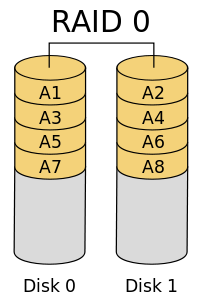
\includegraphics[width=\textwidth]{200px-RAID_0.png}
	\end{column}
	\end{columns}
\end{frame}

\begin{frame}
	\frametitle{RAID 1}
	
	\begin{columns}[T]
        \begin{column}{0.6\textwidth}
		\textbf{Mirror}
		\begin{itemize}
			\item Podaci se kopiraju na više diskova
		\end{itemize}
		\begin{itemize}
			\item Zaštita podataka
			\item Nema povećanja prostora ni performansi
		\end{itemize}
	\end{column}
	\begin{column}{0.3\textwidth}
		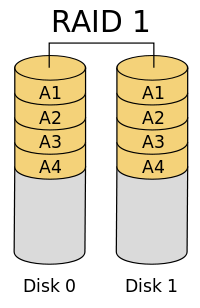
\includegraphics[width=\textwidth]{200px-RAID_1.png}
	\end{column}
	\end{columns}
\end{frame}

\begin{frame}
	\frametitle{RAID 5}
	
	\begin{columns}[T]
	\begin{column}{0.55\textwidth}
		\textbf{Block-striping with distributed parity}
		\begin{itemize}
			\item Podaci se raspodjeljuju na više diskova
			\item Svakom bloku podataka se izračunava paritet i zapisuje na jedan od diskova
		\end{itemize}
		\begin{itemize}
			\item Povećanje prostora
			\begin{itemize}
				\item Potrebno osigurati dodatni prostor za paritet
			\end{itemize}
			\item Povećanje performansi
			\item Zaštita podataka
		\end{itemize}
	\end{column}
	\begin{column}{0.45\textwidth}
		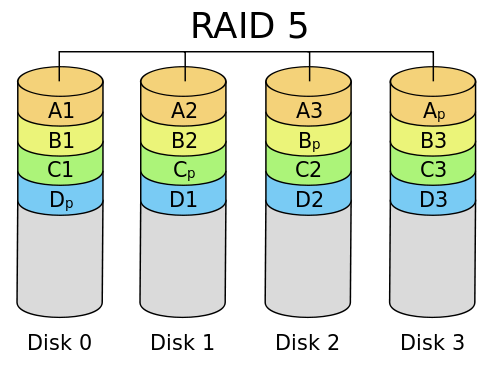
\includegraphics[width=\textwidth]{500px-RAID_5.png}
	\end{column}
	\end{columns}
\end{frame}

\begin{frame}
	\frametitle{Ostali RAID leveli}
	\emph{Nisu u (širokoj) upotrebi}\\
	\vfill
	\textbf{RAID 2}
	\begin{itemize}
		\item Hammingov kod za zaštitu podataka
		\item Dedicirani hard diskovi za zaštitne bitove
	\end{itemize}
	\vfill
	\textbf{RAID 3, 4}
	\begin{itemize}
		\item Paritetna zaštita
		\item Dedicirani hard disk za paritetne bitove
	\end{itemize}
	\vfill
	\textbf{RAID 6}
	\begin{itemize}
		\item Distribuirani zaštitni blokovi
		\item Dvostruki paritetni blokovi
	\end{itemize}
\end{frame}

\subsection{Ugniježđeni RAID leveli}
        \begin{frame}
	\frametitle{RAID 0+1}
	
	\begin{columns}[T]
	\begin{column}{0.55\textwidth}
		\textbf{Stripe, then mirror}
		\begin{itemize}
			\item Podaci se raspodjeljuju unutar jednog polja pa se cijelo polje kopira
		\end{itemize}
		\begin{itemize}
			\item Prednosti RAID 0 na razini jednog polja
			\item Sigurnost RAID 0 polja
		\end{itemize}
	\end{column}
	\begin{column}{0.45\textwidth}
		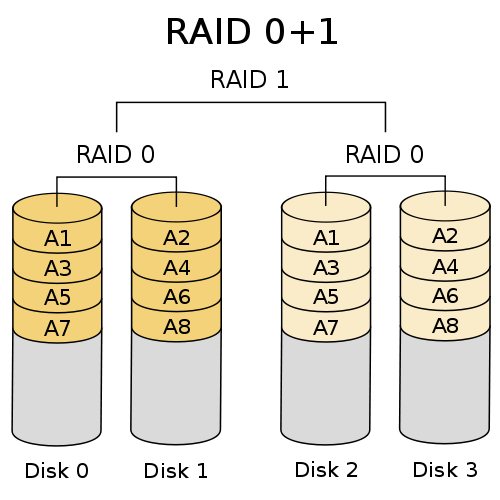
\includegraphics[width=\textwidth]{500px-RAID_01.png}
	\end{column}
	\end{columns}
\end{frame}

\begin{frame}
	\frametitle{RAID 1+0}
	
	\begin{columns}[T]
	\begin{column}{0.55\textwidth}
		\textbf{Mirror, then stripe}
		\begin{itemize}
			\item Podaci se kopiraju unutar jednog polja pa se cijelo polje raspodjeljuje
		\end{itemize}
		\begin{itemize}
			\item Sigurnost RAID 1 na razini jednog polja
		\end{itemize}
	\end{column}
	\begin{column}{0.45\textwidth}
		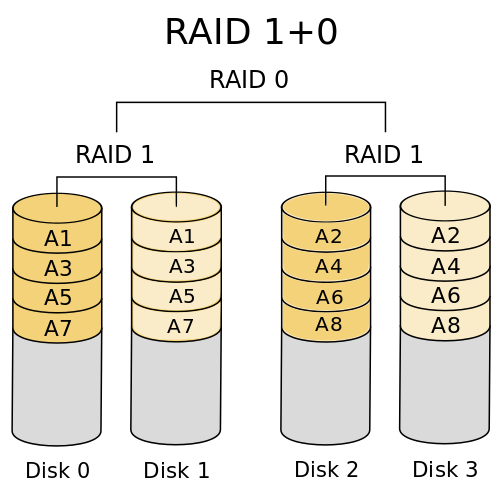
\includegraphics[width=\textwidth]{500px-RAID_10.png}
	\end{column}
	\end{columns}
\end{frame}

\subsection{Hardverski RAID}
\begin{frame}
	\frametitle{RAID kontroler}
	\framesubtitle{RAID ROM}
	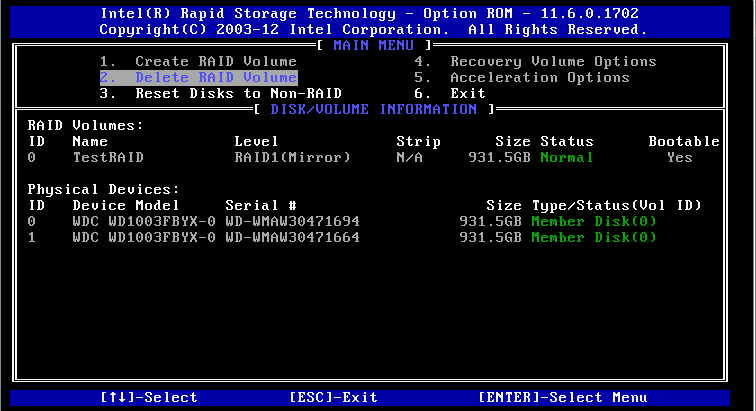
\includegraphics[width=\textwidth]{Intel_RAID.png}
\end{frame}

\subsection{Softverski RAID}
\begin{frame}
	\frametitle{Softverski RAID}
	\textbf{md} - multiple device
	\begin{itemize}
		\item Linux implementacija softverskog RAID-a
		\item Podržava
		\item[] Span, RAID 0, RAID 1, RAID 4, RAID 5, RAID 6, Nested
	\end{itemize}

	\texttt{mdadm}
	\begin{itemize}
		\item[] \texttt{/dev/md*}
		\item[] Particionirana polja
		\begin{itemize}
			\item[] \texttt{/dev/md/md1p1}
			\item[] \texttt{/dev/md/md2p1}
			\item[] \dots
		\end{itemize}
	\end{itemize}
	
	\texttt{/proc/mdstat} - popis inicijaliziranih polja\\
	\begin{itemize}
		\item[] \texttt{mdadm} ne pamti polja pri ponovnom pokretanju
		\item[$\rightarrow$] \texttt{mdadm --detail --scan >> /etc/mdadm.conf}
	\end{itemize}
\end{frame}

\begin{frame}
	\frametitle{RAID boot}
	\textbf{Hardverski RAID}
	\begin{itemize}
		\item[] OS vidi RAID polja kao i fizičke diskove. Nema izravni pristup fizičkim diskovima.
		\item[$\rightarrow$] Bootloader radi kao u konfiguraciji bez RAID-a.
	\end{itemize}
	\vfill
	\textbf{Softverski RAID}
	\begin{itemize}
		\item[] OS vidi fizičke diskove i iz njih gradi polje i logičke diskove.
		\item[$\rightarrow$] Bootloader mora imati podršku za takva polja.
	\end{itemize}
	\vfill
	\textbf{Hardware assisted / \textit{Fake} RAID}
	\begin{itemize}
		\item[] Hibridni model. Kontroler ima ograničenu RAID podršku.
		\item[$\rightarrow$] Bootloader vidi RAID polja kako logičke diskove. Ovisno o hardveru može bootati i bez dodatnih modula.
	\end{itemize}
\end{frame}

\section{LVM}

\begin{frame}
	\topskip0pt
	\vspace*{\fill}
		\begin{center}
			\Huge{LVM}
		\end{center}
	\vspace*{\fill}
\end{frame}

\begin{frame}
	\frametitle{LVM}
	\textbf{Logical Volume Manager}
	\begin{itemize}
		\item Fleksibilnije upravljanje diskovnim prostorom
		\item Implementacija kroz \textbf{device mapper} (dm)
	\end{itemize}
	\begin{itemize}
		\item Moguće dodavanje, uklanjanje i zamjena fizičkih i logičkih diskova za vrijeme rada sustava (čak i bez unmounta)
	\end{itemize}
\end{frame}

\begin{frame}
	\frametitle{LVM arhitektura}
	\textbf{Physical Volume} (PV)
	\begin{itemize}
		\item Particije na fizičkim diskovima
		\item LVM ih dijeli na manje jedinice - \textbf{Physical extent} (PE)
	\end{itemize}
	\vfill
	\textbf{Logical Volume} (LV)
	\begin{itemize}
		\item Logički disk (particija)
		\item LVM ih dijeli da manje jedinice - \textbf{Logical extent} (LE)
	\end{itemize}
	\vfill
	\textbf{Volume Group} (VG)
	\begin{itemize}
		\item Grupira više PV i LV u jednu skupinu radi mogućnosti upravljanja
	\end{itemize}
	\textbf{}
\end{frame}

\begin{frame}
	\frametitle{LVM arhitektura}
	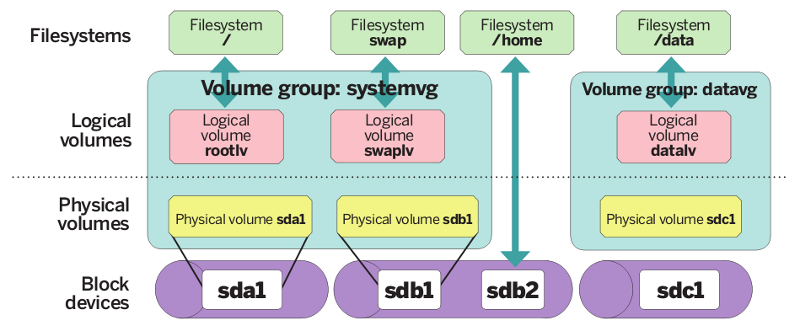
\includegraphics[width=\textwidth]{lvm_arch.png}
	\vfill
	\begin{itemize}
		\item Fizičke particije \textbf{sda1} i \textbf{sdb1} grupirane su u \textbf{systemvg}, a u grupi su stvorene dvije logičke particije: \textbf{rootlv} i \textbf{swaplv}
		\item Particija \textbf{sdc1} je sama u grupi \textbf{datavg}
		\item Particija \textbf{sdb2} zaobilazi LVM i montirana je direktno na \textbf{/home}
	\end{itemize}
\end{frame}

\begin{frame}[fragile]
	\frametitle{LVM}
	\framesubtitle{Primjer}
	\textbf{Kreiranje LVM logičke particije korištenjem dviju fizičkih particija}\\
	\begin{verbatim}
# stvaranje fizičkih particija
pvcreate /dev/sda1 /dev/sdb2 

# stvaranje grupe moja_grupa i dodavanje navedenih particija
vgcreate moja_grupa /dev/sda1 /dev/sdb2 

# Informacije o VG
vgscan
vgdisplay moja_grupa

lvcreate -l 100%FREE -n lvm0 moja_grupa
mkfs.ext3 /dev/lvm-disk/lvm0
	\end{verbatim}
\end{frame}

\begin{frame}[fragile]
	\frametitle{Zašto LVM?}
	\begin{itemize}
		\item Sloj apstrakcije između fizičkih diskova i smještanja podataka u logičke cjeline
		\item Jednostavnije dodavanje i uklanjanje fizičkih diskova
		\item Jednostavnija briga o veličinama i zauzeću particija
		\begin{itemize}
			\item npr. ako je particija premala, bez problema možemo proširiti particiju na drugi disk
		\end{itemize}
		\item Općenito drastično jednostavnija administracija fizičkih diskova
	\end{itemize}
\end{frame}



\section{Kvote}

\begin{frame}
	\topskip0pt
	\vspace*{\fill}
		\begin{center}
			\Huge{Kvote}
		\end{center}
	\vspace*{\fill}
\end{frame}

\begin{frame}
	\frametitle{Kvote}
	\begin{itemize}
		\item Ograničavaju korištenje diskovnog prostora
	\end{itemize}
	\begin{description}
		\item[usrquota] Korisničke kvote
		\item[grpquota] Grupne kvote
	\end{description}
	\begin{itemize}
		\item Obične kvote
		\item \emph{Journaled} kvote
		\begin{itemize}
			\item Vode zapise o promjenama na disku što povećava pouzdanost
		\end{itemize}
	\end{itemize}
	\vspace{1em}
	{\ttfamily \small
		quotacheck: Your kernel probably supports journaled quota but you are not using it.
		Consider switching to journaled quota to avoid running quotacheck after an unclean
		shutdown.
	}
\end{frame}

\begin{frame}[fragile]
	\frametitle{Kvote}
	\framesubtitle{Podešavanje i naredbe}
	Datoteka \texttt{/etc/fstab}
	{\small \begin{verbatim}
# Obicne kvote
/dev/sda2  /home  ext4  defaults,usrquota,grpquota   0  1
# Journaled kvote
/dev/sda2  /home  ext4  defaults,usrjquota=aquota.user,
                 grpjquota=aquota.group,jqfmt=vfsv0  1  1
	\end{verbatim} }
	U prvom direktoriju trebaju biti datoteke \texttt{aquota.user} i \texttt{aquota.group}
	\begin{itemize}
		\item[] \texttt{/home/aquota.user}
		\item[] \texttt{/home/aquota.group}
	\end{itemize}
	\begin{verbatim}
quotacheck -avgum
quotaon -avgu
	\end{verbatim}
\end{frame}

\begin{frame}[fragile]
	\frametitle{Kvote}
	\framesubtitle{Podešavanje i naredbe}
	{\footnotesize \begin{verbatim}
# repquota -a

*** Report for user quotas on device /dev/md0
Block grace time : 7 days ; Inode grace time : 7 days
                         Block limits                 File limits
User          used       soft     hard  grace   used  soft hard  grace
-----------------------------------------------------------------------
root    --       52         0        0            10     0    0
veljko  -- 25585028  40000000 40000000          1123     0    0
cetko   --  5162460  40000000 40000000            49     0    0
marin   --  6498572  10000000 20000000           183     0    0
deni    --  5903852  10000000 20000000           528     0    0
lovro   --  3649796  10000000 20000000            19     0    0
matej   +- 11334792  10000000 20000000  2 days   646     0    0
	\end{verbatim}}
\end{frame}

\begin{frame}[fragile]
	\frametitle{Kvote}
	\framesubtitle{Podešavanje i naredbe}
	\begin{description}
		\item[Soft limit] Aktivacija \emph{grace period-a} za vrijeme korisnik još može koristiti prostor
		\item[Hard limit] Limit nakon kojeg korisnik nema mogućnost pisanja po disku
	\end{description}
	\vspace{1em}
	{\footnotesize \begin{verbatim}
# edquota cetko

Disk quotas for user cetko (uid 1001):
 Filesystem         blocks        soft        hard inodes soft hard
 /dev/md0          5162460    40000000    40000000     49    0    0
	\end{verbatim}}
\end{frame}

\section{Napredne mogućnosti}

\begin{frame}
	\topskip0pt
	\vspace*{\fill}
		\begin{center}
			\Huge{Napredne mogućnosti filesystema}
		\end{center}
	\vspace*{\fill}
\end{frame}

\begin{frame}
	\frametitle{Napredne mogućnosti filesystema}
	\framesubtitle{File attributes}
	File attributes
	\begin{itemize}
		\item Određuju poseban režim rada filesystema kod određenih datoteka / direktorija
		\item Vrste atributa određene su odabirom filesystema
		\item Za ext2 i novije ext sustave postoje naredbe za upravljanje atributima
		\item[] \texttt{lsattr}, \texttt{chattr}
	\end{itemize}
	\vspace{1em}
	Neki od ext2 atributa:
	\begin{itemize}
		\item[a] Append only - dopušta samo dodavanje sadržaja fajlu
		\item[A] No atime updates
		\item[c] Compressed - automatska kompresija fajla
		\item[i] Immutable - brani svaku promjenu fajla (\textbf{čak i od roota!})
		\item[s] Secure deletion - pri brisanju prebriše prostor nulama
		\item[u] Undeletable - omogućuje vraćanje obrisanih podataka
		\item[] ...
	\end{itemize}
\end{frame}

\begin{frame}[fragile]
	\frametitle{Napredne mogućnosti filesystema}
	\textbf{Primjer}\\
	\vspace{1em}
	Kreirajte datoteku koju korisnik \texttt{root} neće moći izbrisati korištenjem naredbe\\
	\verb|# rm -f file.txt|\\
	\vspace{1em}
	{\footnotesize Rješenje je napisano bijelim slovima}\\
	\vfill
	\textcolor{white}{Postaviti immutable atribut}
\end{frame}

\begin{frame}
	\frametitle{Napredne mogućnosti filesystema}
	\framesubtitle{Access Control Lists (ACL)}
	Access Control Lists (ACL)
	\begin{itemize}
		\item Proširenje UNIX dozvola
		\item Dodjeljivanje različitih dozvola različitim korisnicima i grupama
	\end{itemize}
	\vspace{1em}
	\texttt{setfacl}, \texttt{getacl}
	\vspace{1em}
	\begin{itemize}
		\item Filesystem mora biti mountan s opcijom \texttt{acl}
	\end{itemize}
\end{frame}

\begin{frame}[fragile]
	\frametitle{Napredne mogućnosti filesystema}
	\framesubtitle{Extended attributes}
	Extended attributes
	\begin{itemize}
		\item Parovi \texttt{kljuc:vrijednost} koji se mogu po volji pridijeliti datotekama
		\item Oprez prilikom kopiranja datoteka
		\begin{itemize} 
			\item uobičajene naredbe za kopiranje ne čuvaju extended atribute
		\end{itemize}
		\item Proučiti man stranice
	\end{itemize}
	Klase atributa
	\begin{multicols}{2}
		\begin{itemize}
			\item security
			\item system
			\item trusted
			\item user
		\end{itemize}
	\end{multicols}
	{\footnotesize \begin{verbatim}
		$ setfattr -n user.test -v "podatak" file.txt
		$ getfattr -d file.txt
		# file: file.txt
		user.test="podatak"
		\end{verbatim}}
\end{frame}

\begin{frame}[fragile]
	\frametitle{Napredne mogućnosti filesystema}
	\frametitle{Extended attributes}
	Capabilities
	\begin{itemize}
		\item Koncept ograničavanja mogućnosti izvršnih datoteka
		\item Cilj je izbjeći korištenje \textit{setuid} bita ostavljajući izvršnoj datoteci privilegirani pristup nekim dijelovima sustava
	\end{itemize}
	\vspace{1em}
	{\footnotesize \begin{verbatim}
	$ getcap /bin/ping
	/bin/ping = cap_net_raw+ep
	\end{verbatim}}
	\begin{itemize}
		\item Capabilities se zapisuju kao extended atributi
	\end{itemize}
	{\footnotesize \begin{verbatim}
	$ getfattr -d -m "^security\\." /bin/ping
	# file: bin/ping
	security.capability=0sAQAAAgAgAAAAAAAAAAAAAAAAAAA=
	\end{verbatim}}
\end{frame}

\begin{frame}[fragile]
	\frametitle{Loop devices}
	\begin{itemize}
		\item Interpretacija običnih datoteka kao uređaja
		\item Datoteci se dodjeljuje \emph{loop} uređaj u \texttt{/dev} folderu kojem se pristupa kao običnom disku
	\end{itemize}
	\begin{itemize}
		\item Datoteka može sadržavati datotečni sustav
	\end{itemize}
	\vfill
	\textbf{Primjer stvaranja loop device-a}:
	\begin{verbatim}
	# Prazna 100MiB datoteka
	dd if=/dev/zero of=device.img bs=512 count=2048
	
	losetup /dev/loop0 device.img
	mkfs -t ext3 /dev/loop0
	mount -t ext3 /dev/loop0 /mnt/image
	\end{verbatim}
\end{frame}

\section*{}
\begin{frame}
	\frametitle{Literatura}
    \url{http://www.ufsexplorer.com/und_fs.php}
    \url{http://www.tldp.org/HOWTO/Filesystems-HOWTO-6.html}
    \url{http://www.nongnu.org/ext2-doc/ext2.html}
    \url{https://www.linux.com/news/software/applications/8208-all-about-linux-swap-space}
	\texttt{man mdadm}
	\url{http://www.ducea.com/2009/03/08/mdadm-cheat-sheet/}
	\vfill
	\url{http://debian-handbook.info/browse/wheezy/advanced-administration.html}\\
	\url{https://www.howtoforge.com/linux_lvm}
	\url{https://wiki.archlinux.org/index.php/Software_RAID_and_LVM}\\
	\url{http://www.tuxradar.com/content/lvm-made-easy}
	\vfill
	\url{https://wiki.archlinux.org/index.php/disk_quota}
\end{frame}

\end{document}
